\languecmncn

\chapter*{前言}

%\section{缘起}

在中国西南部,云南与四川交界处生活着一个知名的族群——摩梭人。\footnote{本导言由第一作者米可撰写。}它奇特的民族风俗使它名扬天下,然而,它的语言研究还远远跟不上它的名气。作为一名语音学家找到了摩梭语言就如同进入了阿拉丁的宝库:摩梭语音的丰富多彩,尤其是声调在整个语法系统里所起的核心作用,独特而又迷人。

本词典的第二作者是一位充满独特个人魅力的摩梭阿妈——拉他咪打史拉姆。1950年出生的这位阿妈,差不多与新中国同年龄,她身上的故事就是摩梭人今天与昨天的缩影。
她在云南省丽江市宁蒗县永宁镇\footnote{中国云南省丽江市宁蒗彝族自治县的永宁乡于2019年2月11日改设为永宁镇。}阿拉瓦村(平静村)独自养育了四个儿女,其中一位就是摩梭著名学者拉他咪王勇(拉他咪·达石)。有幸结识拉他咪王勇先生与他亲爱的母亲是这本词典得以与世人见面的关键,在此向他们表示最深切的感谢。

本引言分为三个部分:(i)简要介绍摩梭语以及为编制词典而开展的合作(§\ref{sec:lang}),(ii)用户指南(§\ref{sec:guide}),最后(iii)浅谈濒危语言词典编制工作的意义。

\section{永宁镇阿拉瓦村摩梭语的调查}
\label{sec:lang}

永宁摩梭语,自称\phonologie{nɑ˩-ʐwɤ˥}。该语言的\texteeng{Ethnologue}代码为\texteeng{\textsc{nru}}\parencite{lewisetal2016},其\texteeng{Glottolog}代码是 \texteeng{\textsc{yong1270}}\parencite{Nordhoff2012}。
1979年,语言学家和即仁、姜竹仪对纳西与摩梭地区进行了调查,将摩梭语归类为纳西语东部方言\parencite[4, 104--116]{heetal1985}。将{纳西语}分为东部和西部两种方言这一说法,一开始是谨慎提出的初步想法:是基于1950年代中华人民共和国境内语言调查资料的一种工作假设。

\begin{quotation}
我们从现有的语言和人文材料来加以分析和比较,将纳西语初步分划为西部和东部两个{方言}。不过时间短促,经验不足,这样划分不知是否符合客观现实情况{\dots}\parencite[120]{heetal1988}
\end{quotation}

{\noindent}上述提到的西部{方言}大体上与14-18世纪丽江纳西族统治的区域相对应。东部{方言}区位于其东部和东北部,横跨长江,在今宁蒗、盐源、木里、盐边等县境内。和即仁、和志武又将东部{方言}分出三个土语:永宁坝、瓜别和北渠坝。

这一分类后来成为中国学术研究的标准,还被收录在“世界少数民族语文研究院”(\texteeng{Summer Institute of Linguistics},1983年改名为\texteeng{SIL International})的语料库“民族语:全世界的语言”(\texteeng{Ethnologue: Languages of the World},又译为“民族语言网”)当中\parencite{gordon2005}。{纳西}语过去在“民族语”资料库中的语言代码为\texteeng{\textsc{nbf}},涵盖了上述所有语中,即纳西语、摩梭语的所有{方言}。自2010年起,{纳西}语的东部{方言}在“民族语”资料库中被赋予了自己的条目代码,\texteeng{\textsc{nru}}(等于拼音写法\texteeng{“Narua”}的缩写)。原来的语言代码\texteeng{\textsc{nbf}}被分为两类:{纳西}语得了\texteeng{\textsc{nxq}}这一新代码,对应中文术语中的“{纳西}语西部{方言}”;摩梭语得了\texteeng{\textsc{nru}}这一代码,对应中文术语中的“{纳西}语东部{方言}”。等于说,至今国内外还使用着和即仁、姜竹仪、和志武关于方言的分类(只是用的名称不同而已)。

根据早期调查,讲摩梭语的总人口大约有四万人\parencite[107]{heetal1985}。2020年代精通摩梭语的人数估计要少得多,摩梭语逐渐被汉语所取代。自20世纪 90年代以来,特别是进入21世纪以来,永宁地区已成为一个重要的旅游目的地,产生了深刻的社会变化\parencite{milan_tourisme_2019}。如法国诗人伊夫·博纳富瓦(\textefra{Yves Bonnefoy})的直觉不谋而合:

\begin{quote}
    旅游业就像洪水携带着残骸一样蔓延开来。即使是最偏远的村庄也被它弄得支离破碎,它在寺庙最隐秘的房间里大肆宣扬其空洞、傲慢的公式:唉,这些都是我们西方文化的典型刻板印象。广告小册子不是任何人的言论;它们往往迫使所到之处的居民从外面看自己,按照懒惰的游客希望的方式讲述自己的故事,用华丽的图片取代自己的直觉和记忆,以迎合游客的口味。(伊夫·博纳富瓦, \textefra{\emph{L'Inachevable. Entretiens sur la poésie}, 1990-2010.} 巴黎:\textefra{Albin Michel}出版社,2014年,232页。)
\end{quote}

摩梭语的调查研究在这种背景下显得尤为重要。我希望,在实地录制并逐步转写、翻译和注释的录音资料,将成功地保存和传播我老师(本词典合著者)的声音。她为了当代人和后人将宝贵的录音录像资料公之于众。这些资料的价值不仅在于抽象意义上让人类语言和社会研究有据可查,供类型学和历史参考:摩梭文化,还有摩梭阿妈拉他咪打史拉姆本人,本身就是非常值得我们关注、详细了解的。这一点,我再借一下我们这边诗人的说法来表达。

	\begin{quote}
    ‘世界’,对我们来说,首先难道不就是人们开垦和耕种过的田地吗?那么看,我们用的词,也就是在粗糙冷漠的空间里能肯定、铭刻并表达我们的存在感的一种方式。或者这样说吧:词言,不要当是处理一般抽象概念的手段。每个词是一种窗口,让我们可以理解人类与其存在的具体地点之间的关系。那么,词汇不是我们所说的“大自然”的百科全书。词是通向一片可入住的土地(相当于斯特凡·马拉梅所说的‘住居地’)的大门,在那里我们可以安居乐业。在这片土地上,我们可以宾至如归,熟悉的名字为我们指明方向,为我们开辟视野。这么看,每一次相遇都将是我们命运的一个新部分出现,而不是为某些科学概括提供素材的抽象事件。我们觉醒的意识应将新相遇视为一种新鲜开放的开始(尽管时间的飞逝夺走许多这样的可能性)。我们不应该把活生生的遭遇从我们的言语中抹去,把它们仅仅当作某种抽象永恒规律的例子。(伊夫·博纳富瓦,\textefra{«La fleur double, la sente étroite: la nuée»},重印于\textefra{\emph{La Vérité de parole et autres essais}},巴黎:伽利玛出版社,1995年,566-567页。)
\end{quote}


\subsection{摩梭语研究综述}
\label{sec:previousstudiesofthenalanguage}


中文的历史资料对几个世纪前永宁使用的语言提供了迷人的一瞥。1286年成书的{《元一统志》}中有‘丽江’和‘永宁’这两个地名的汉语音译,分别记录为“样渠头”和“楼头”。记载于14世纪的韵书{《中原音韵》}中的汉语,“头”的声母是清音,不是浊的;但柯蔚南对八思巴文的重构里,它被构拟为*\phonétique{dəw} ,与现在的摩梭语和{纳西}语具有相同的浊辅音\parencite{coblin2007}。“楼头”被构拟为*\phonétique{ləw dəw},与今天的永宁摩梭语(\phonologie{ɬi˧di˩})和{纳西}语(\phonologie{ly˧dy˩})明显同源。这个词的发音本身就足以证明该地名至少可以追溯到元代。它还为中国历史{音韵学}争议的一个焦点提供了{证据},即元代的汉语(北方官话)保留了浊塞音\parencite[487]{jacquesetal2011}。

在20世纪之交的探险家笔记里,有关语言的信息不很丰富,因此这里就不再讨论这些文献。读者可参考\textcite{michaudetal2010}及该文中所列举的文献。


\subsubsection{《纳西语简志》中关于摩梭语的材料}
\label{sec:heandjiang1985}

和即仁和姜竹仪二位先生在1985年出版的《纳西语简志》中,主要介绍了丽江平坝的{方言},但该书也提供了永宁摩梭语的一个词表,以及对其音系、句法和{方言}多样性的一些观察(107–116页;另见\textcite{jiang1993})。
《{纳西}语简志》里的语音转录没有进行音位归纳,而且可能前后不完全一致。他们在{单音节词}上记录了四个调类:一个升调(底中\phonétique{¹³},\phonétique{˩˧}), 一个中{平调}(\phonétique{³³},\phonétique{˧}), 一个降调(中底\phonétique{³¹},\phonétique{˧˩}), 和一个高{平调}(\phonétique{⁵⁵},\phonétique{˥}),而其实有六个{单音节词}声调类别(词调),即底中(LM)、底高(LH)、中(M)、底(L)、高(H)、还有中高(MH)\parencite{michaud2017}。和即仁和姜竹仪对摩梭语的研究主要是基于同{纳西}语的对比,他们两位先生都会说{纳西}语(和即仁本身就是母语人:丽江县金山乡漾西林红村人,姜竹仪是第二语言学习者)。纳西语的{单音节词}有四种声调对立:高、中、低(语音上表现为低降)和升。在记录永宁摩梭语时,和即仁与姜竹仪没有将低升调和中升调区别开。此外,他们还报告了双音节词的头音节上中{平调}(\phonétique{³³},\phonétique{˧})与高{平调}(\phonétique{⁵⁵},\phonétique{˥})的区别,而事实上并不{存在}这样的对立。当然,也可能是他们调查的{方言}与同我合作的语言老师所讲的{方言}有很大差别,但是他们的调查词表与本书报告的数据之间有很强的语音相似性,所以这种可能性不大。马提索夫就曾经指出,基于短期田野考察的数据进行音位处理和声调分析时,由于音位分析不完整,很容易在不同的作者之间产生很大的差异\parencite[329]{matisoff2004}。

回到永宁摩梭语的中{平调}M和高{平调}H,在本书描写的{方言}里(阿拉瓦{方言}),这两种词调在{{单独}}发音时,就中和为一个中{平调},M。根据{布拉格}学派的音系分析方法,该声调可以称其为{中和}音位(\texteeng{archiphoneme})。\footnote{{\texteeng{\emph{Archiphoneme}}}这个概念好像尚未有固定的汉语翻译,我们试着称作“{中和}音位”,那可能是最简单清楚的叫法,因为中和音位就是音位中和化的成果:它来自音位对比在某些位置被中和。\texteeng{Archiphoneme},也可以试着称作“共性音位”,反映了它作为抽象音系单位代表了不同音位的共同显著特征。其它的翻译选择还包括“泛音位”或“音位上位素”之类。}
这个中和调的实际发音在声调空间的上半部分可以{自由变体},只要它高于低调(L)。所以调查者如果假设这个语言中{单音节词}上{存在}调高平H和中平M的对立,那么他就可以听到好像支持自己这个假设的音高差异。这种预设会影响语言学的观察,此情况也发生在我田野调查的早期阶段:在我最初的转录中,也分了{单音节词}上的调高平H和中平M。后来我发现,它们{单独}发音时并没有对立,只是自由变体。在阿拉瓦{方言}中,中调(M)和高调(H)是两种不同的词调,但只有放在某些合适的语境里才能反映出来,比如添加系动词时。因此,和即仁和姜竹仪将中{平调}M和高{平调}H的对立定义为基本词调的对立(即一个{单音节词}孤立时候的发音)是站不住脚的(除非如上文所述,我们所讨论的{方言}声调系统之间{存在}相当大的差异)。词条“地”被转写为高{平调}\phonétique{lv̩˥},而实际上它是一个中{平调}\phonétique{lv̩˧}(本书用双斜线来表示底层词调形式(\texteeng{lexical tone}),与表层音系形式的单斜线形成区别)。“人”被转写为中{平调}\phonétique{xĩ˧},这个词{单独}读音时的确是中{平调},但它在不同语境中的表现显示它的底层词调实际是高调H(我的转录是:\phonologie{hĩ˥})。

和即仁和姜竹仪的数据中,低(降)和低升调的分布让我困惑。因为在我调查的这个{方言}中,没有一个{单音节词}孤立发音时表现为低调。例如“平原、平地”“水”和“鹅”分别被他们转写为\phonétique{dy˧˩}、\phonétique{dʑi˧˩} 和 \phonétique{o˧˩}。而这三个词在我的记录中声调是不同的:“平原、平地”是LH调,“水”是L调,“鹅”是LM调。我猜测,在和即仁和姜竹仪的发音人的话语里,L是LH的(相对不常见的)自由变体。或者是他们调查的词条汇聚了多个发音人的数据,所以{方言}材料不同质。《纳西语简志》里有关纳西语的描写也有类似的情况:作者介绍的资料有青龙镇的{方言}(今长水),这是姜竹仪先生的老师和志武的故乡,也有一些数据是和即仁先生自己的漾西{方言}。由于他们没有对每条数据做出标注,很难判断语料具体来自哪个{方言}。

和即仁和姜竹仪对元音和辅音的转录也{存在}一些问题,他们的记录在一些方面像是早期的田野调查笔记。比如,鼻音只在两个音节里出现:\phonétique{xĩ}(例如“人”这个词,他们转录为\phonétique{xĩ˧};我的记录是:\phonologie{hĩ˥})和\phonétique{ɣə̃r}(唯一的例子是“骨头”,他们转录为\phonétique{ʂa˧ɣə̃r˧};我的转录是:\phonologie{ʂæ˩ɻ̩̃˩}),而本书一共调查到八个不同的鼻音韵母。还有一点不同的是小舌辅音与软腭音的对立,他们没有转录,这种差异可能是由于和即仁、姜竹仪所描写的{方言}的音位数量本身就比本书所描写的{方言}的音位数量要少,也有可能是他们当时没有区分出一些{存在}对立的音位,这也不是不可能的。

另一方面,和即仁、姜竹仪转录的一些元音对立可能也站不住脚。他们的词条中包含\phonétique{li}(如\phonétique{li˧}“看”)和\phonétique{lie}(如\phonétique{lie˩˧}“茶”)的区别。在我的数据中,“看”和“茶”的声母与韵母是一样的。有时候元音\phonologie{i}会滑向\phonétique{e}音,略微呈现为双元音,听感上接近\phonétique{lie},这就解释了有些调查人在整体了解摩梭语的元音系统之前,有时候会转写为\phonétique{i},有时转写为\phonétique{ie}。当然我要再次声明,理论上讲也有可能在和即仁、姜竹仪调查的{方言}变体中,它们确实是两个不同的音位。

\subsubsection{一篇亲属称谓研究,包含一些音系讨论:\textcite{fu1980}}
\label{sec:fu1980astudyofkinshipterms}

语言学家傅懋勣于1979年5至6月随和即仁、姜竹仪去永宁调查。在甲波瓦村(\phonologie{dʑɤ˩bv̩˧-ʁwɤ˩} )收集数据,研究亲属称谓。他的论文首先在第十二届国际汉藏语言学年会(巴黎,1979年)上宣读,之后又相继以中文和法文发表\parencite{fu1980,fu1983}。这篇论文证明了摩梭家庭结构多么有吸引力,在专业的人类学家之外还能引起语言学家的兴趣。该文的附录中有语音转写,可以在本书所介绍的较为成熟的音位分析的基础上回头看傅先生的转写。此处仅回顾一些有突破性的观察,例如:傅先生注意到了小舌音\phonologie{q}、\phonologie{qʰ}和\phonologie{ʁ}与软腭音的对立。他还记录了近音\phonétique{ɹ},指出它可以出现在元音前面(即作为声母),也可以{单独}构成一个音节;这与本书的分析一致,本书选择的转写符号是卷舌音\phonologie{ɻ}{\kern2pt}。

然而,傅懋勣的巧妙见解之外,也有一些令人费解的提议。例如,他的一组小舌辅音中还包括一个擦音\phonétique{χ},如果进行更仔细的分析就应该会发现这个擦音它与软颚音没有对立,迄今为止记录的所有纳西语和摩梭语{方言}都是这样的情况。可想,在三位先生联合的实地考察中,假设当时和即仁、姜竹仪观察到了检查了傅懋勣所转写的资料,他们就很可能会对\phonétique{χ}音位存疑,而他们的(正确)怀疑可能也会延伸到傅懋勣对小舌\phonologie{q}和\phonologie{qʰ} 作为不同的音位的新发现。和即仁、姜竹仪没有接受傅懋勣对小舌音的分析,也有可能来自他们二位对纳西语音系的了解。纳西语也有小舌音\phonétique{q}和\phonétique{qʰ},这两个音是软颚塞音的语音变体。这就会让纳西语的使用者推断在纳语组的其他语言中,小舌音也是软颚音音位的变体。此外,摩梭语\phonologie{k}和\phonologie{kʰ}与\phonologie{q}和\phonologie{qʰ}对立的音系环境也不很多。

傅懋勣的记音还有其他几个问题:1)他认为,\phonétique{u}、\phonétique{v̩}和\phonétique{z̩}这三种韵母,都{存在}有两种,一种普通韵母,一种喉化韵母(共六个不同的韵母);2)除了近音韵母\phonétique{ɹ},傅懋勣还认为有三个儿化元音;3)他认为\phonologie{i}与\phonologie{e}这两个元音有对立但\phonologie{i}在舌尖音与舌尖-齿音之后实际发音为\phonétique{e}。总而言之,傅先生的音位归纳还不算全稳定的。至于声调,傅懋勣将其分为中升、高平、中降三类,这个分类表明他选择从零开始,立起自己对摩梭语声调系统的分类,而不是以纳西语的声调为基础。这种方法非常合理,很值得称道的。但是摩梭语声调系统不是一般的复杂,所以并不奇怪傅先生没有辨识出所有的声调类别(词调)。该报告中这些零碎的问题也从某些方面说明为什么和即仁、姜竹仪在撰写他们1985年的书籍时,没有充分利用傅懋勣的材料。然而,值得我们记住的是,在1979年能去永宁进行实地考察本身就是一项了不起的成就。



\subsubsection{杨振洪的《摩梭语概况》}
\label{sec:yang2009}


杨振洪的《摩梭语概况》最初是在2006年以中文出版\parencite{yang2006d},之后由利伯缇·利兹(Liberty Lidz,汉语名字:李力)翻译为英文,与作者进行了一些修改,英文版2009年问世出版\parencite{yang2009}。杨振洪老师是阿布瓦村(\phonologie{ə˧bv̩˧-ʁwɤ˧})人。这篇论文的体例大致遵循了和即仁、姜竹仪对{纳西语}的描写。有些语音和音系的部分需要再进一步的分析,比如,需要认识到小舌和卷舌塞音的音位地位。在声调方面,他的分析是以{纳西语}的四个调为基准,这必然会有一些不足。笔者与杨振洪在2011年进行过非正式交流,我向他展示了在该{方言}中实际上{存在}更多的声调类别。杨振洪与其他许多研究人员一样,使用的是类似研究汉语{方言}声调时用到的音节声调系统,这套系统不足以完整地描写摩梭语的声调。相同的问题也出现在对{普米语}的研究中,研究人员在了解了其他类型的声调系统后,例如了解了对{日语}{方言}的研究之后,才最终实现了对{普米语}声调进一步的认识\parencite{ding2001,ding2006,jacques2011a}。



\subsubsection{词汇材料}
\label{sec:dictionary2013}

《摩梭语常用词句荟萃》\parencite{zhibaetal2013}从语义领域编撰词汇及句子。该书作者一位是泸沽湖地区的母语人,另一位是云南大学的语言学博士生。他们的田野调查覆盖了永宁平原和泸沽湖地区,以永宁平原为主(第2页)。

这本书中不准确的转写太多,以至于无法把它视为一个可信的参考文献。对于这个团队的语言学工作者(第二作者)来说,确认清浊对立是个很大挑战,因为她受到的训练主要集中在对外汉语教学的理论和实践上。因此就出现了将山名\phonologie{kɤ˧mv̩˧˥}转写为\phonétique{gə⁵⁵mu⁵⁵}的情况,将声母记作浊音(第17页和书中的其他地方)。这座山的中文名字叫格姆山,或许拼音、\texteeng{\emph{Gemu}}在这里产生了影响。与其相反,形容词\phonologie{dʑɤ˩\textsubscript{b}} “好”被转写为\phonétique{tɕɑ¹³},声母被记作清音。还有一些音位,比如小舌音,没有被转写出来。


\subsubsection{口述文献汇编:摩梭祷文}
\label{sec:collectionsoforalliteraturenaritualtexts}
在永宁平原,藏传佛教(格鲁派)与当地负责传统宗教仪式的达巴(\phonologie{dɑ˧pɤ˧})并存。与纳西人不同的是,摩梭人的仪式没有被书面下来,尽管他们有一些在占卜时用来计算日子的文字(参见\textcite{yang1985}和\textcite[163-189]{lidazhu2015})。缺少书也部分解释了为什么摩梭达巴受到的关注比纳西东巴少。与丽江相比,永宁的规模和社会政治影响都要小得多,而且直到20世纪后期交通不便、进入到该地区困难,这也解释了为什么几乎没有人费力去整理和记录摩梭的这些口头仪式的内容。

由一位母语人出版的双语合集中\parencite{azeming2013}包含以下内容:1)用汉字标出每个音节的近似语音;2)用国际音标转写每个音节;3)提供每个音节的中文注释;4)将每一行翻译成中文(一行一般包含五个、七个或八个音节)。这本书,估计对已经很熟悉摩梭语的读者才能有帮助,因为他们只要参照汉语拼音系统的转写习惯,就能够辨识出文中的对应发音。例如,\phonétique{p}、\phonétique{t}、
\phonétique{k}显然分别用于转写送气音\phonétique{pʰ}、\phonétique{tʰ}、\phonétique{kʰ},就像汉语拼音中的p、t、k一样。如:“白色”一词声母在摩梭语里是送气的,但在该书中被转写为\phonétique{puə}(第4页)。这本书里面没有标声调。

在2010年前后,拉他咪王勇(拉他咪达石)启动了一个摩梭达巴经记录计划,旨在出版大量包含视频、翻译和注释的仪式合集。《摩梭达巴口诵经典》(数字多功能光盘[\texteeng{DVD}]7碟装)以内部资料的形式问世(制作时间:2011年3月-2012年8月,制作:云南省社科院宁蒗民族文化研究所,田野报告人:打发鲁若,导演、田野访问人、摄像:拉他咪王勇、总顾问:木桢、李宝山、胡志海),是有重大意义的资料。

深入研究摩梭仪式,同时与纳西仪式进行对比,一定可以更加深入地理解摩梭人的文化(参见\textcite{mathieu2015},以及该书中列举的参考资料)。这项研究需要精通{藏语}文学,深入了解{藏}传佛教,以及其他专业领域的技能,我的专业知识还远远不够。{藏}传佛教与摩梭信仰相互接触,一些例子来自20世纪的调查报告。僧侣和{达巴}能够和平共处、分工明确。杀猪时人们会叫{达巴}来举行仪式,而历法上规定的重要日子则请僧侣。有些重要的事件要同时请僧侣和{达巴},例如葬礼。这种和平共处,以及双方共同参加仪式而产生的接触机会,显然导致了某种程度的趋同和融合。可以看出,摩梭的{达巴}受到了佛教僧侣高度仪式化行为的影响。他们在准备自己的仪式时会很注重细节,要提前备好所有必要的用具,如酥油、蜡烛、水和不同粮食的面,这很像佛教的僧侣。相比之下,{彝}族的毕摩(仪式主持人的称谓)则习惯于在仪式进行的过程中突然提出要求,索要物品和配件,似乎完全依灵感行事(拉他咪王勇,私人交流,2008年)。{达巴}的手势也变得和僧侣的手势较接近。反过来,一些僧侣也在学习摩梭达巴的占星术,这是达巴的能力之一。


\subsubsection{利伯缇·利兹的《{永宁纳}语(摩梭语)的描写语法》\parencite{lidz2010}}
\label{sec:lidz2010}
迄今为止,对永宁摩梭语最全面的描述和分析是利伯缇·利兹(\texteeng{Liberty Lidz},汉语名字:李力)的博士论文\parencite{lidz2010}《{永宁纳}语(摩梭语)的描写语法》。他描写的是泸沽湖畔落水村的摩梭语,该论文基于深入的实地调查,描写了该语言的形态句法,并且还有150多页经过转写和注释的口述材料。
关于声调问题,杜玫瑰(\texteeng{Roselle Dobbs})与喇明清提出了:“落水纳阮(纳语)的声调系统需要进一步分析。目前的音系分析采用了三个调[即高、中、底],但大部分资料似乎可以从两个调[即高与底]的视角来重新分析。论文里有提到{存在}有丰富的连词变调,但这些现象没有给出详细的描述和说明”\parencite{dobbsetal2016}。参考语法的研究通常会遗留一些韵律问题,比如声调或者重音的处理\parencite[26]{zeitoun2007}。

在近几年中,对以前未记录的方言声调系统的研究取得了明显进展\parencite{a2016,dobbsetal2016,fily_documentation_2022}。

\subsection{调查的方言与合作者(语言顾问)}

永宁坝子位于中国西南部,云南和四川交界处,北纬 27°50',东经 100°41'(见地图)。永宁紧邻泸沽湖(\phonologie{lo˧ʂv̩˩-hi˩nɑ˧mi˧}),一个面积约五十平方公里的湖泊,尽管海拔较高(约 2800 米),但这里的小气候适合农耕。

除非另有说明,所有语料均来自第二作者:拉他咪打史拉姆女士。她1950年出生在永宁寺附近阿拉瓦村(云南省丽江市宁蒗彝族自治县永宁镇\footnote{云南省丽江市宁蒗彝族自治县永宁乡于2019年2月11日更名为永宁镇。}阿拉瓦村)。该语言变种的\texteeng{Glottolog}代码为\texteeng{\textsc{yong1288}},有别于泸沽湖畔的方言区(后者的代码为\texteeng{\textsc{lata1234}})。在地图\ref{map:1-1}中用星形符号表示阿拉瓦村的位置。

\begin{figure}
	\centering
	\caption{永宁地区的地图。设计:\textefra{Jérôme Picard}。信息来源:\texteeng{Geofabrik, ASTER GDEM,OpenStreetMap}。}
	\includegraphics[width=.68\textwidth]{Lien vers images/PDF_CMYK_1point4.pdf}
	\label{map:1-1}
\end{figure}

之所以选择只在一个地方工作,而且主要仅与一位顾问(发音合作人)工作,是因为我最初将研究重点放在声调系统上。摩梭地区的方言多样性相当大(比纳西语方言内部差异大得多)。不同村庄的声调系统差异明显,而且这种地域多样性与不同社会群体和不同世代之间的明显差异结合在一起。显而易见,要先完成的任务就是对一个人所说的语言进行深入描述和分析(当然同时按照机会对其它方言进行一些尝试性的调查)。合作进行得很顺利,以至于拉它米女士2024 年接受了将她的名字作为本卷合著者的建议。

其他发音合作人的数据在词典中用两个字母的首字母表示,在表\ref{table:ConsultantsTable}中最左边一栏提供。表中标明了与我的数据库中发言人代码的对应关系,如:‘F5’等于本书的‘Gi’,指的是郭给若女士。摩梭发音合作人在这些发音人代码的编号是不连续的(七位的编号分别为F4、F5、F6、F22与M18、M21、M23,而不是F1至F4与M1至M3),因为他们是作为纳语组三种语言(即纳西语、摩梭语与木里水田话)发音合作人名单分配的。

\begin{longtblr}[
  caption = {合作人},
  label = {table:ConsultantsTable}
]{
  colspec = {X[0.6,l,m]X[1.1,l,m]X[l,m]X[l,m]X[0.6,l,m]X[0.3,l,m]},
  rowhead = 1
}
  \hline
  {名字首字母} & {名字(拉丁字母)} & {名字(国际音标)} & {名字(汉字)} & {出生年} & {代码} \\
  \hline
        La & Latami Daeshi Lhamu & \phonologiebis{lɑ˧tʰɑ˧mi˥ ʈæ˧ʂɯ˧-lɑ˩mv̩˩} & 拉他咪打史拉姆 & 1950 & F4 \\
        Gi & Gisso & \phonologiebis{ki˧zo˧} & 郭给若 & 1973 & F5 \\
        Qi & Qiddeu & \phonologiebis{tɕʰi˧ɖv̩\#˥} & 郭园芝 & 1987 & F6 \\
        Sg & Siggeema & \phonologiebis{sɯ˧gɯ˧mɑ˧} & 思格玛 & 1987 & F22 \\
        Da & Latami Daeshi Daedeu & \phonologiebis{lɑ˧tʰɑ˧mi˥ ʈæ˧ʂɯ˧-ʈæ˩ʈv̩˩} & 拉他咪王勇 & 1972 & M18 \\
        Jj & Ho Jjacee & \phonologiebis{ho˧dʑɤ˧tsʰe˥} & 何甲泽 & 1942 & M21 \\
        Dd & Ddeezzhi  & \phonologiebis{ɖɯ˩ɖʐɯ˧} & 何独知 & 1974 & M23 \\
  \hline
\end{longtblr}

随着时间的推移,发音合作人的小圈子逐渐扩大。第一个联系人是拉他咪王勇老师,他热心地在村里寻找语言顾问。这种寻找起初并没有结果,于是是他的母亲(拉他咪打史拉姆女士)同意担任顾问教师的角色。她始终是语言调查工作的标准发音人、主要资料来源和日常对话伙伴。她的一位儿媳(郭给若)和后者的一个侄女(郭园芝)也同意帮忙。后来,拉它米女士的一个堂兄(何甲泽先生)和他的儿子(何独知)也参与了调查。思格玛女士来自瓦拉比村,她的主要贡献在于与杜玫瑰女士一起参加和对工作,讨论摩梭语语音、语义、语法、方言学、拼音系统等问题。

在没有任何固定总体计划的情况下,长期积累起来的这个合作人小组并没有根据任何特定标准进行平衡,也没有声称它在任何意义上具有代表性。尽管如此,我们还是可以描述这个‘发音人样本’的一些特点。

就世代而言,样本显示出一定的多样性。七位并不都属于同一世系,而是分属三个连续的世代。拉他咪打史拉姆女士(本卷的合著者)出生于1950年,与何甲泽先生属于同一代人。下一代的代表有拉它米女士的儿子拉他咪王勇、郭给若和何独知(何甲泽先生的儿子)。郭园芝和思格玛更年轻,可以被视为属于第三代。

语言和文化的关系方面:

\begin{itemize}
    \item 拉他咪打史拉姆女士对摩梭文化的浸润最深,她在阿拉瓦村连续居住了六十年(从出生到 2010年)。
    \item 郭给若和何独知属于留在村里的下一代(截至2024年,他们仍住在村里),对他们来说,本地汉语(西南官话)是从小就能流利使用的语言,接近于第二母语。
    \item 拉他咪王勇毕生致力于摩梭文化研究,对摩梭文化有着深厚的感情。他日常与母亲一起使用摩梭语。他能讲流利的母语(摩梭语)。\footnote{他录的八段视频可在网上查阅:\href{https://doi.org/10.24397/pangloss-0007734}{永宁与摩梭人};\href{https://doi.org/10.24397/pangloss-0007740}{“摩梭”这一族称的历史与意义};\href{https://doi.org/10.24397/pangloss-0007730}{成长:讲述演讲者在摩梭人家庭中的生长过程,青年时代及其人生历程};调查语言的客人:回顾与语言学家十二年的合作,\href{https://doi.org/10.24397/pangloss-0007736}{上}与\href{https://doi.org/10. 24397/pangloss-0007738}{下};\href{https://doi.org/10.24397/pangloss-0007742}{摩梭研究回顾};\href{https://doi.org/10.24397/pangloss-0007728}{文化精神的延续:关于摩梭人的文化记忆};\href{https://doi.org/10.24397/pangloss-0007732}{火塘:关于火塘在摩梭文化中的意义}。他的著作包括\textcite{latami2006}、\textcite{latami2009}、\textcite{latami2016}等等。} % Séparer manuellement les cas compliqués comme celui-là.
    \item 何甲泽先生曾在永宁地区的不同地方生活过,这自然导致他的语言与那些出差经历不那么丰富的人的语言之间存在一定的距离。我特别感谢他在部分失聪的情况下仍努力参与语言调查工作。
\end{itemize}

语言学家的一个永恒目标和希望就是让发音合作人尽可能密切地参与到对其语言的研究中来。本书由主要顾问(拉他咪打史拉姆女士)共同署名的决定符合这一逻辑。她的儿子拉他咪王勇并没有等到与我(米可)的交流才进入学者圈子,作为一名专门研究摩梭文化的民族学家,他对本书的重要贡献是基于他的学术才能,而不仅是他作为母语使用者的身份。

此外,还有两位重要合作者,即杜玫瑰阿姨(\texteeng{Roselle Dobbs},新西兰人,摩梭名字:独玛拉搓)。她以及她的摩梭朋友和合作者,除了赋予本词典的拼写法之外,从我对永宁摩梭语的研究开始以来一直提供大量信息、更正和建议。区勄狐(\textefra{Benjamin Galliot},法国人),自2016年以来一直按照最高的计算和排版标准编辑本部词典,对细节和整体结构都极为关注。

\subsubsection*{阿拉瓦村摩梭语,是方言、次方言还是土语呢?}

在此,我们不试图界定阿拉瓦村摩梭语方言的地理边界,也不定义‘方言’、‘次方言’、‘土语’等等之间的区别。“阿拉瓦方言”这一标签,足够作为在这一地点收集的语料的标记。我们并不试图将这一方言列入包含所有摩梭方言的某个综合清单中。

不过,可能还是会有人提出,为这一方言(土语)编纂词典这一事实,就使阿拉瓦摩梭语在仍然非常稀少的当代摩梭语词汇学中占据了重要位置。从这个角度来看,词典中提供的拼音文字具有较高的价值,因为它旨在实现方言之间的某种平衡:它并不只基于一种方言(或以某个特定的发音人作为标准:作为权威参考),细见\textcite{dobbs_ortho_2018}。

\subsection{语言调查与词典编辑工作的总计划和时间顺序}

我2006年到永宁调查摩梭语,开始的初衷只是进行音系分析,但却惊奇地发现摩梭声调不仅是单纯的音系问题,同时与语法有着千丝万缕的联系。这一发现,促使我开始对摩梭语进行全方位的研究。研究方法以搜集来的长篇语料为蓝本,在搜集语料的同时以长篇语料中的词汇为基准汇集成本部词典。

编辑词典的过程一般都很漫长,以至于这个话题成为了笑话的素材。例如,在狄更斯的《大卫·科波菲尔》中,一位老教授就因为着手进行一项超出他能力范围的词典项目而遭到嘲笑。
\begin{quotation}
    我们的班长精通数学,他曾计算过,按照校长的计划和进度,他考虑新编的词典需要多少时间才能完工。他的结论是,从校长的最近一个生日,即六十二岁生日算起,将需要一千六百四十九年来完成。(狄更斯,《大卫·科波菲尔》,1850年,第十六章。)
\end{quotation}

然而,濒危语言调查这一领域的压力恰恰相反,时间通常非常紧迫。工作必须尽快取得具体成果,即合同资助研究项目所设想的“可交付成果”。
\begin{quotation}
    由于项目受到资金、人员和时间等有限资源的制约,项目的组织方式必须使词典编纂者即使在很短的时间内也能完成一部有用的作品。\parencite[“濒危语言社区的词典编纂”:][42]{mosel_dictionary_2004}。
\end{quotation}

本词典的编辑过程篇向漫长,作风属于相当传统的田野调查方法。在语言学田野调查的经典传统中,语言描述应包括词典、语法和文本集(长篇语料集)\parencite{michaud2012_yongning}。语言学田野调查包括“进入使用某种语言的社区,从流利的母语使用者那里收集数据,分析数据,并创造一份由语法、语料集(文本集)和词典组成的综合描述”\parencite[12]{dixon2007}。语法、语料集和词典被称为语言调查三件宝\parencite{sun2007}。\footnote{长篇语料就是我囊中最大的宝贝,历时十八年搜集而来的近二十个小时的资料及部分资料的逐句标注翻译,已经全部在线公开,请见“泛语语料库”(\texteeng{Pangloss Collection}),\href{https://pangloss.cnrs.fr/}{pangloss.cnrs.fr}。}按照这种方法,本卷中的词汇数据是在对永宁阿拉瓦村进行全面实地考察的过程中收集的。2006年、2007年、200 年和2009年前往实地考察。2011-2012年,拉他咪打史拉姆女士在丽江城定居照顾孙女,于是调查在丽江继续,时间有满满一年。我2013年、2014 年、2018年和2024年也到丽江与她合作,逗留时间较短。

一开始用词表诱导一些词汇,列出一个初步的词表,然后在记录和转写故事的过程中逐步扩充和修正词汇数据库。不诱导大量词汇的一个缺点是,增加新词是一个缓慢的过程。因此,词条数量到现在还是很有限:大约有三千条(目前的具体数字为\obtenircompteur{total})。另一方面,将重点放在文本收集上的一个好处是,可以通过上下文来帮助澄清新词的含义,也为与语言顾问进一步讨论其用法提供了基础。

\begin{quotation}
    受访者在被要求翻译一个他们不理解的单词时可能会感到非常尴尬。而假如他们因为忘记了母语的对应词而无法翻译这个单词,又更丢脸。

    由于这类重要的问题,通过翻译引出的单词总是需要再通过翻译回原文(如:汉语或英语)进行反查确认。民族语词汇的含义可能比外文词汇的含义更宽或更窄,而且两种语言中的词汇各会有其多义性,因此它们的含义只有部分相似。\parencite[44]{mosel_dictionary_2004}
\end{quotation}

应《汉藏语系词典》(STEDT)数据库管理团队的建议,截至2011年的词表已存入此数据库\parencite{stedt}。同年,在向柏霖老师(\textefra{Guillaume Jacques})和\textefra{Aimée Lahaussois}老师的推动下,制定了使词表更接近正式词典标准的计划。2012年,他们申请的一个项目被国家研究协会(\textefra{Agence Nationale de la Recherche})所接受,并于2013年启动:\textefra{HimalCo}项目(\textefra{\textsc{anr-12-corp-0006}})。

词典是需要一直补充修改的工具,一直是“进行中的工作”。按照软件开发所使用的模式,对词典的连续版本进行编号。主要版本预计最多每隔几年发布一次。下文按时间顺序介绍了迄今为止已完成的版本。中文版本见表 \ref{table:versionsZH},英文版本见表\ref{table:versionsEN},法文版本见表\ref{table:versionsFR}。

\begin{longtblr}[
  caption = {为汉语读者设计的版本},
  label = {table:versionsZH}
]{
  colspec = {X[0.8,l,m]X[0.8,l,m]X[l,m]X[1.4,l,m]},
  rowhead = 1
}
  \hline
  版本号 & 日期 & 网址 & 软件 \\
  \hline
  1.2 & 2018年3月 & \href{https://shs.hal.science/halshs-01744420v1/}{halshs-01744420v1} & \href{https://github.com/CNRS-LACITO/Lexika}{Lexika(编程语言: Python)} \\
  2.0 & 2024年 & \href{https://shs.hal.science/halshs-01744420v2/}{halshs-01744420v2} & \href{https://gitlab.com/BenjaminGalliot/JLexika}{JLexika(编程语言: Julia)}\\
  \hline
\end{longtblr}

\begin{longtblr}[
  caption = {为英语读者设计的版本},
  label = {table:versionsEN}
]{
  colspec = {X[0.8,l,m]X[0.8,l,m]X[l,m]X[1.4,l,m]},
  rowhead = 1
}
  \hline
  版本号 & 日期 & 网址 & 软件 \\
  \hline
  1.0 & 2015年9月 & \href{https://shs.hal.science/halshs-01204638v1/}{halshs-01204638v1} & \href{https://github.com/CNRS-LACITO/HimalCo/tree/master/dev/lib/pylmflib-1.1}{PyLMFlib} \\
  1.1 & 2016年11月 & \href{https://shs.hal.science/halshs-01204638v2/}{halshs-01204638v2} & \href{https://github.com/CNRS-LACITO/HimalCo/tree/master/dev/lib/pylmflib-1.1}{PyLMFlib} \\
  1.2.1 & 2018年4月 & \href{https://shs.hal.science/halshs-01204638v3/}{halshs-01204638v3} & \href{https://github.com/CNRS-LACITO/Lexika}{Lexika(编程语言: Python)} \\
  1.2.2 & 2018年7月 & {该版本没有存入HAL资料库。} & \href{https://github.com/CNRS-LACITO/Lexika}{Lexika(编程语言: Python)} \\
  2.0 & 2024 & \href{https://shs.hal.science/halshs-01204638v4/}{halshs-01204638v4} & \href{https://gitlab.com/BenjaminGalliot/JLexika}{JLexika(编程语言: Julia)} \\
  % \pnrubis{pò-ko-kabu} & \pnrubis{po-ko-kabun} & jeudi(3 j. [avant le] jour sacré) \\
  % \pnrubis{pò-tru kabu} & \pnrubis{po-ru-kabun} & vendredi(2 j. [avant le] jour sacré) \\
  % \pnrubis{po-xè kabu} & \pnrubis{po-xe kabun} & samedi(1 j. [avant le] jour sacré) \\
  \hline
\end{longtblr}

\begin{longtblr}[
  caption = {为法语读者设计的版本},
  label = {table:versionsFR}
]{
  colspec = {X[0.8,l,m]X[0.8,l,m]X[l,m]X[1.4,l,m]},
  rowhead = 1
}
  \hline
  版本号 & 日期 & 网址 & 软件 \\
  \hline
  1.0 & 2015年9月 & \href{https://shs.hal.science/halshs-01204645v1/}{halshs-01204645v1} & \href{https://github.com/CNRS-LACITO/HimalCo/tree/master/dev/lib/pylmflib-1.1}{PyLMFlib} \\
  1.1 & 2016年11月 & \href{https://shs.hal.science/halshs-01204645v2/}{halshs-01204645v2} & \href{https://github.com/CNRS-LACITO/HimalCo/tree/master/dev/lib/pylmflib-1.1}{PyLMFlib} \\
  1.2.1 & 2018年4月 & \href{https://shs.hal.science/halshs-01204645v3/}{halshs-01204645v3} & \href{https://github.com/CNRS-LACITO/Lexika}{Lexika(编程语言: Python)} \\
  2.0 & 2024年 & \href{https://shs.hal.science/halshs-01204645v4/}{halshs-01204645v4} & \href{https://gitlab.com/BenjaminGalliot/JLexika}{JLexika(编程语言: Julia)} \\
  % \pnrubis{pò-ko-kabu} & \pnrubis{po-ko-kabun} & jeudi(3 j. [avant le] jour sacré) \\
  % \pnrubis{pò-tru kabu} & \pnrubis{po-ru-kabun} & vendredi(2 j. [avant le] jour sacré) \\
  % \pnrubis{po-xè kabu} & \pnrubis{po-xe kabun} & samedi(1 j. [avant le] jour sacré) \\
  \hline
\end{longtblr}

\subsubsection{1.0版和1.1版:遵循“词汇标记框架”(LMF)标准}

在项目的第一阶段,团队采用了“词汇标记框架”(LMF)标准,这是一种专为机器可读词典设计的格式\parencite{francopoulo2013,romary2013}。\textefra{Céline Buret}是一名计算机科学工程师,她参加了项目团队两年(2014年11月至2015年10月)。她编写了脚本,用于将词典数据从田野语言学工具箱\texteeng{Toolbox}的格式(\texteeng{MDF}格式)转换为符合“词汇标记框架”(\texteeng{LMF})标准的\texteeng{XML}玛。她编辑了一个脚本库:\texteeng{PyLMFlib},\texteeng{\emph{Python LMF library}}。2015年,词典的1.0在线版和PDF版发布,同时发布的还有MDF格式的源数据库。2016年发布的1.1版也使用了相同的计算机脚本库。

\subsubsection{Lexika软件和Lexica词典集}

“词汇标记框架”在2013年制定时的一个局限性逐渐显现出来了:它对条目所能包含的内容施加了限制。属于不同词类的子条目需要设置单独的条目。例如,\phonologie{lɑ˧-kʰv̩˧˥}既可以表示‘虎年’,也可以表示‘属虎’。从语言学家的角度来看,在同一个条目中设立两个子条目是可取的。但这两个词条的词类是不同的:‘虎年’是名词,而‘属虎’是谓词。在“词汇标记框架”中,这种情况需要设置两个不同的词条,这一要求与词典学的普遍做法不符。

2016年,计算机科学工程师区勄狐(\textefra{Benjamin Galliot})在法国国家科学研究中心口传语言与文化研究所(\textefra{CNRS-LACITO})的一份定期(6个月)合同下工作,编写了一个新的软件,即\textefra{\emph{Lexika}}。按照引进古希腊语词根的新法语词汇的习惯,这个词用K这个字母,不同于词典系列的名字,\textefra{\emph{Lexika}}\parencite{lexica2017},后者按照引进拉丁语词产新词的拼法习惯用C那个字母。这样,能防止软件与词典系列之间的混淆。

2017年年中,区勄狐(\textefra{Benjamin Galliot})对Lexika 软件进行了全面改造\parencite{galliot:2017:lexika},新版本称为JLexika,因为它是用Julia语言编写的。这项工作为区勄狐的一项个人挑战,他想掌握一种自己感兴趣且更符合自己编程风格的编程语言。在他的工作过程中提出的一些问题,以及为解决这些问题而开发的解决方案,已在\textcite{galliot:2023:lexikaproblématiques}中列出。

2017年年底,在与\textefra{Laurent Romary}老师和\textefra{Mathieu Mangeot-Nagata}老师交换意见时,他们确认区勄狐的选择是正确的,即:遵守“词汇标记框架”(\texteeng{LMF})标准确实没有明显的好处,而且需要繁琐的变通方法才能达到预期效果。除其他益处外,新格式还有助于条目之间的交叉引用,例如指出同义词、反义词、词源等等。

当时,区勄狐(\textefra{Benjamin Galliot})个人在\textefra{JLexika}上的工作是基于一种没有任何硬标准的格式,因此\textefra{Lexika}软件的XML模型在2018年初明确远离了\textefra{LMF}标准。\textefra{Lexika}的目的,就是满足语言学家的期望和愿望。在整个工作过程中,他始终关注的问题是保持高度的内部一致性,从而使计算机探索和分析达到最佳效果。换句话说,要避免在没有任何实际内部必要性的情况下屈从于先验强加的约束。

多年后,当区勄狐(\textefra{Benjamin Galliot})以公务员身份重返法国国家科学研究中心时,他认为继续开发JLexika更为合适,因为JLexika功能更强大、更稳健。这项工程的理念在其最新版本中发挥到了极致,可以用这样一句话来概括:“考虑到语言和语言学家的多样性,我们如何才能建立词典创建模型?”\textefra{Lexika}的格式,可以在一个共同的基础上(见\url{https://hal.science/LEXICA})根据每部词典的需要进行定制。通过XSL样式表,可以将\textefra{Lexika}格式与文本编码倡议(\textefra{TEI})标准兼容,但\textefra{Lexika}格式存在的理由在于其广泛的自定义功能,可最大限度地适应语言和语言学家的需要。如:\textefra{Lexika}可以设置所需的层次结构(子条目和或多义词、各种细分)、各级可以带有丰富的文本(各种样式、链接、语言和文字),以及所有必要的其它信息(如:注释、标签、百科信息、词源解释等等),这些都可以附加到结构的各个层次。勄狐的参与程度非同一般,这意味着每部词典在结构、开发和排版方面都成为独一无二的精品,以便最好地适应所描述语言的具体特点和词典编纂者的愿望。从1.2版开始,词典从总体结构到最小的排版细节都是他一手打造的。他对一丝不苟的审美观的承诺鼓励我们加倍努力,让词典的内容也达到最高水平。他建立的灵活、动态的处理链允许随着调查的进展更新XML和PDF文件,这也促进了数据库的丰富。

在\textefra{Lexika}处理链中,词典的PDF版本由XML文件生成,而XML文件本身则由源文件生成,源文件仍为MDF格式。

中间版本(如1.2.1,继1.2之后)随着工作的进展而生成,并通过\texteeng{GitHub}存储库提供。\footnote{\url{https://github.com/alexis-michaud/na/tree/master/DICTIONARY}}

2.0版本起,拉他咪打史拉姆女士成为合著者,反映了她对词典的核心角色。人类学家皮艾木(法国人,外文名\textefra{Pascale-Marie Milan}:帕斯卡尔-玛丽·米兰,摩梭名字:瑸妈拉姆)也成为合著者,这不仅反映了她的重要作用,还反映词典的重要未来发展方向,即追求民族学与人类学方面的高经制度。

% \section{为什么编辑单方言词典而不编辑多方言词典}
% 因为方言(土语)之间差异大,所以严格以一个地方,一个人的发音为标准音。如:粗绳索,永宁阿拉瓦村是\phonologie{bæ˧mi˧}。这个词与‘鸭子’同音。而左所舍夸村的摩梭语里,\phonologie{bæ˧mi˧}表示鸭子,\phonologie{bæ˧mi˩}才表示粗绳索,大绳索。




\section{用户指南}
\label{sec:guide}

Lexica系列词典旨在将(i)用户浏览词典的可读性与(ii)适合语言处理的计算机可读编码相结合。因此,词典以多种格式提供:
\begin{itemize}
    \item PDF文档
    \item HTML格式的在线词典
    \item Toolbox/MDF格式的数据库(主文件)
    \item 通过\textefra{Lexika}软件生成的XML文件。
\end{itemize}

数据库可以从在线软件源代码托管服务平台\texteeng{GitHub}中以两种格式获取:

\begin{itemize}
    \item 区勄狐(\textefra{Benjamin Galliot})设计的模型的XML文件
    \item MDF格式的主文件,可以用“工具箱软件包”(\texteeng{SIL Toolbox})打开
\end{itemize}

便携式文档格式(PDF)有三种语言设置,以满足不同语言群体的需求: 中文版(本版本,\href{https://shs.hal.science/halshs-01744420}{halshs-01744420})、英文版(\href{https://shs.hal.science/halshs-01204638}{halshs-01204638})和法文版(\href{https://shs.hal.science/halshs-01204645/}{halshs-01204645})。

首先介绍数据库结构,然后介绍排版选择。

\subsection{数据库结构}

只要看一眼下面的XML代码摘录,就能回答有关数据库结构的大部分问题:见代码示例\ref{code:LexikaXML}。

\begin{lstlisting}[language=XML, caption=说明词条结构的XML代码摘录, label=code:LexikaXML]
<EntréeLexicale identifiant="ⓔhĩ˧-ʈʂɤ#˥">
  <Lemme>
    <Forme>hĩ˧-ʈʂɤ#˥</Forme>
    <Ton>#H</Ton>
    <Orthographe>hinzhe</Orthographe>
    <FormeDeSurface>hĩ˧ʈʂɤ˧</FormeDeSurface>
  </Lemme>
  <PartieDuDiscours langue="eng">n</PartieDuDiscours>
  <ListeDeSens>
    <Sens>
      <DomainesSémantiques>
        <DomaineSémantique langue="fra">société</DomaineSémantique>
        <DomaineSémantique langue="eng">society</DomaineSémantique>
      </DomainesSémantiques>
      <Définitions>
        <Définition langue="eng">Family member belonging to the same lineage (on the mother's side).</Définition>
        <Définition langue="cmn">亲戚:有共同祖先(祖母)的家人</Définition>
        <Définition langue="fra">Membre de la famille de même lignage (du côté maternel).</Définition>
      </Définitions>
      <Gloses>
        <Glose langue="eng">family_members_of_same_lineage</Glose>
        <Glose langue="cmn">亲戚</Glose>
        <Glose langue="fra">membre_de_la_famille_de_même_lignage</Glose>
      </Gloses>
      <Exemples>
        <Exemple>
          <Original langue="nru">hĩ˧-tɕʰɯ˧ - hĩ˧-ʈʂɤ#˥</Original>
          <Traduction langue="eng">same meaning: the family members belonging to the same lineage</Traduction>
          <Traduction langue="cmn">同上:亲戚,有共同祖先(祖母)的家人</Traduction>
          <Traduction langue="fra">même sens: les gens de même lignage</Traduction>
        </Exemple>
      </Exemples>
      <RelationsSémantiques>
        <RelationSémantique>
          <Cible identifiant="ⓔhĩ˧-tɕʰɯ#˥">hĩ˧-tɕʰɯ#˥</Cible>
          <Type langue="fra">synonyme</Type>
        </RelationSémantique>
      </RelationsSémantiques>
    </Sens>
  </ListeDeSens>
</EntréeLexicale>
\end{lstlisting}

% \begin{figure}[ht!!]
%     \centering
%          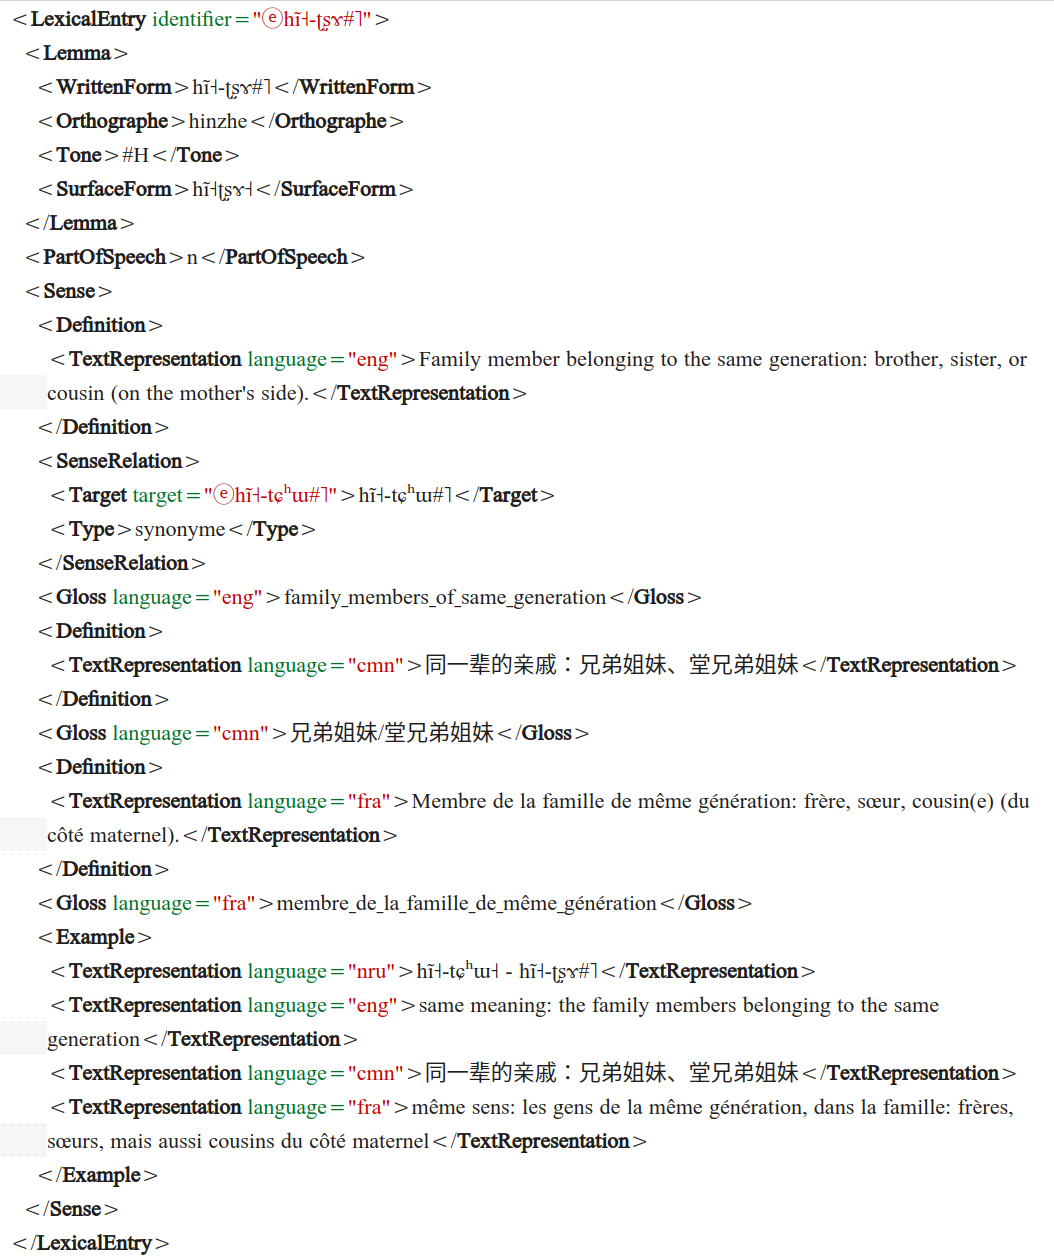
\includegraphics[width=\textwidth]{images/LexikaXML.png}
%         \caption{Lexika XML词典数据库结构的示例条目}
%         \label{fig:LexikaXML}
% \end{figure}

词典由词条(\texteeng{\emph{lexical entries}})组成。每个词条都有一个计算机标识符。该标识符不显示在词典的\texteeng{PDF}版本中,因为其作用是让计算机进行操作,而不是让人眼识别。该标识符由特殊字符\textecode{ⓔ}和单词的发音(此处为 \phonologie{hĩ˧-ʈʂɤ\#˥})组成。

词条的“词目”(\texteeng{\emph{lemma}})部分包括四项信息:
\begin{itemize}
    \item 其深层(抽象)语音形式。声调符号系统使用特殊符号(\$ 和 \#)来区分不同类型的高声调。关于该系统的完整解释可参见专著《永宁摩梭语的声调》,该书可在线开放获取\parencite[80-90]{michaud2017}
    \item 声调(“本调”)
    \item 拼音写法(由杜玫瑰女士提供)
    \item 表面语音形式(对应于该词在单独发音时的实际发音)
\end{itemize}

接着是词类(该词的形态句法类别)。

然后是对词义的描述。从一个封闭的术语列表(法语和英语)中提供语义域的分类:该词属于‘社会’、‘房子’、‘身体’、‘植物’、或是‘动物’等等的语义领域。这是一种粗略的划分,部分依赖于形式,部分依赖于语义。我没有尝试使用英语WordNet数据库中的精细语义分类法,在该数据库中,名词、动词、形容词和副词被归类为认知同义词集\parencite{fellbaum2005}。

提供了中文、英文和法文定义。在少数情况下,还提供了摩梭语的定义。用所研究的语言编写释义的过程非常有用\parencite{dingemanse_folk_2015},本词典的合著者也擅长此道;不过,此类释义仍然很少,因为迄今为止用于这项工作的时间太少。

词典还提供了释义,以便将来对文本(长篇语料)进行系统释义。本词典大多沿用\textcite{lidz2010}所推荐的释义。

例句也被视为“词义”的组成部分,因为它们有助于解释该词的含义。每个例子都包括摩梭语转写与三种目标语言(汉、英、法)的翻译。许多示例都附有注释,注释带有关于其语言学领域的说明:语义学、句法学、形态学、语音学、声调学\footnote{声调学的编码与语音学不同,因为它在文献和研究工作中发挥着重要作用。}或是方言学。%这些附加信息会出现在PDF文件中(除非注释在数据库中带有\textecode{print={\"}n{\"}}标签)。

带有“历史”标签的注释的功能在于记录并解释从最早的田野工作到当前版本的分析历史。这些注释记载了词条内容变化的日期以及支持该变化的论据。例如,\phonologie{ŋwɤ˧pʰæ˧˥}‘瓦片’这个词条有注释,表示‘瓦片’最初是用 M.H声调转写的,而且两个音节都有\phonologie{æ}元音:\phonétique{ŋwæ˧pʰæ˥}。该注释解释说,在第一个音节中出现\phonétique{æ}元音事实上是元音和谐的结果。约有一半的词条有此类信息。这种有时迂回的历史似乎与大多数读者无关,因此没有出现在PDF中。

同义词等语义关系和词源有其编码。在词典目前的状态下,标注为“词源”的信息主要包括双音节词或多音节词与其组成语素之间的联系:例如,指出\phonologie{æ˧ʂæ˧-pi˧mv̩˧˥}‘传说故事’由两个词组成:\phonologie{æ˧ʂæ\#˥}‘从前’和\phonologie{pi˧mv̩˥\$}‘成语、俗语、格言’。

\subsection{字典词条的结构}
\label{sec:structure_of_entries}

每个条目都以音标开头--这里是\phonologie{ɑ˩pʰv̩\#˥}。声调是根据专著《永宁摩梭语的声调》中分析的声调类别来标注的\parencite[80-90]{michaud2017}。
在其右侧的斜线(斜线)之间有一个表面形式,是该词的单独发音,通常称为“引用形式”。这个音标形式是简明好读的国际音标,声调用表面声调。这种形式(此处为:\phonétique{ɑ˩pʰv̩˥})可由任何具有国际音标知识的人读出,无需了解永宁摩梭语中本调(词汇中的声调类别)与表面声调的映射关系。表面形式中去掉了特殊符号:\phonologie{\$}和\phonologie{\#}(用于区分各种类型的高调),也去掉了重叠形式中的波浪號(\phonologie{\hspace{0.5em}\raisebox{-0.6ex}{\~}})等特殊符号。量词前加‘一’这个数字,因为量词不能单独说出。词缀与附着词则都不标明表面形式。
% Précédemment utilisé : (\phonologie{\raisebox{-0.6ex}{{\:}\~}\:})

此外,还提供了拼音写法,用杜玫瑰与熊燕二位设计的拼音系统\parencite{dobbs_ortho_2018}。如:此处为\emph{opu}。拼音由杜玫瑰女士2017年开始添加入资料库。一个重要的原则是:拼音写法不是与阿拉瓦村的发音直接对应。本词典里词条的国际音标转写均基于第二作者的方言,而拼音则是杜玫瑰,熊燕及与她们合作的人作为跨方言拼音系统而提出的。鉴于方言的高度多样性,提出一种能被多种方言使用者接受的转写法意味着一些妥协。例如,只标注了低声调(L)(在单音节词末尾用字母\emph{q}标注),因为在设计拼音时发现,低声调与其它声调相比,从方言学的角度看是更稳定的。

后面有关于不同合作人的发音信息。发音人编码后标注‘同’来表示其发音与词典的合著者(即标准发音人)的发音相同。如果有差异,就显示为其发音的国际音标转写。

词类标注,用一组简单的标签来表示,如表\ref{table:PartsOfSpeech}所示。

\begin{longtblr}[
  caption = {词类},
  label = {table:PartsOfSpeech}
]{
  colspec = {X[0.9,l,m]X[0.9,l,m]X[0.9,l,m]X[1.3,l,m]},
  rowhead = 1
}
  \hline
  {缩写} & {英语} & {汉语} & {词典里此词类的条目数量}  \\
  \hline
        \texteeng{\textsc{adj}} & \texteeng{adjective} & 形容词 & \obtenircompteur{adj} \\
        \texteeng{\textsc{adv}} & \texteeng{adverb} & 助词 &\obtenircompteur{adv} \\
        \texteeng{\textsc{clf}} & \texteeng{classifier} & 量词 & \obtenircompteur{clf} \\
        \texteeng{\textsc{clitic}} & \texteeng{clitic} & 附着词 & \obtenircompteur{clitic} \\
        \texteeng{\textsc{cnj}} & \texteeng{conjunction} & 连接词 & \obtenircompteur{cnj} \\
        \texteeng{\textsc{disc.ptcl}} & \texteeng{discourse particle} & 语气助词 & \obtenircompteur{disc.ptcl} \\
        \texteeng{\textsc{ideophone}} & \texteeng{ideophone} & 状貌词 & \obtenircompteur{ideophone} \\
        \texteeng{\textsc{intj}} & \texteeng{interjection} & 感叹词 & \obtenircompteur{intj} \\
        \texteeng{\textsc{n}} & \texteeng{noun} & 名词 & \obtenircompteur{n} \\
        \texteeng{\textsc{num}} & \texteeng{numeral} & 数词 & \obtenircompteur{num} \\
        \texteeng{\textsc{postp}} & \texteeng{postposition} & 后置词 & \obtenircompteur{postp} \\
        \texteeng{\textsc{pref}} & \texteeng{prefix} & 前缀 & \obtenircompteur{pref} \\
        \texteeng{\textsc{prep}} & \texteeng{preposition} & 介词 & \obtenircompteur{prep} \\
        \texteeng{\textsc{pro}} & \texteeng{pronoun} & 代词 & \obtenircompteur{pro} \\
        \texteeng{\textsc{suff}} & \texteeng{suffix} & 后缀 & \obtenircompteur{suff} \\
        \texteeng{\textsc{v}} & \texteeng{verb} & 动词 & \obtenircompteur{v} \\
  \hline
\end{longtblr}

单词的本调标注出现在词类的后面。语音转录中已经包含了这一信息,但将其单独重复出来有助于读者可以一目了然搜索本调。

接着有中文、英文和法文的定义。

示例主要分为三类。“词典示例”是在田野调查中收集的,专门用来给某个词举例。第二类为从长篇语料中复制的例子,除了转写和翻译以外,词典里还提供连接,这样方便去查原资料、参考其上下文、听原来的录音文件(资料保存于“泛语语料库”,一个开放存取的在线档案库:\href{https://pangloss.cnrs.fr/}{pangloss.cnrs.fr})。第三类仅是向在线档案库中示例的超链接,这些示例似乎对相关词语的研究特别有启发性,但在词典中全文转载似乎并不十分恰当。

许多示例附有注释,每个注释带有关于其语言学领域的说明:语义学、句法学、形态学、语音学、声调学\footnote{声调学的编码与语音学不同,因为声调学在摩梭语研究工作中发挥着重要作用。}或是方言学。这些附加信息出现在PDF文件中(除非注释在数据库中带有\textecode{\texttt{print="n"}}这样的标签)。

为研究特定词语组合的声调而引出的示例前面都标有“(音系资料)”这一说明。谚语和俗语标注为“(谚语)”。

最后,还有向相关词的链接,如同义词、反义词、词源等等。对于名词,还标出最常用的量词(此处为\phonologie{mi˩})。一般不再使用的旧词标注为:“【用法】古词”。

从双音节中提取的单音节词根用符号†表示。那些词条没有提供表面形式,因为这些单音节形式目前在摩梭语中并不使用。

汉语借词有其特殊的标注:“(汉语借词)”。词典没有系统地收集汉语借词,但将文本中出现的所有借词都加入了词典。

\subsection{从词条到在线文本的链接}

如§\ref{sec:structure_of_entries}所述,部分示例节选自“泛语语料库”中的摩梭语资料(录音文件)。“泛语语料库”(\texteeng{Pangloss Collection})是一个开放存取的在线档案馆\parencite[参见][]{michailovskyetal2014}。通过没份资料的“数字对象唯一标识符”(\texteeng{Digital Object Identifier}),可从PDF文件一键链接到在线档案库中实例的确切位置。

除了这些手工挑选的链接之外,未来改进的前景还包括在资源之间建立系统的动态链接。这样,词典、长篇语料(就是构成语言资源核心的文本)和语法出版物可以越来越多地相互连接起来\parencite{maxwell2012}。文本中的真实例句构成了解释一个词的用法的最佳资源。与文本中的实例相比,词典中目前提供的例句数量很少,而且其使用背景不一定十分清楚,尽管我们努力为实地考察中记下的词例提供背景信息。目前还无法提供一个词在文本中出现的完整列表。这项工作需要给文本加工:要生成一份完整的列表,需要对收集到的所有文本进行完整的逐词翻译与标注。


\section{词汇学的研究意义}
\label{sec:recherche}

词汇学一直被认为是语言科学中的边缘学科,其任务好像限于进行简单的清点工作。塞缪尔·约翰逊(\texteeng{Samuel Johnson})在其1755年出版的《英语词典》(\texteeng{\emph{Dictionary of the English Language}})序言中哀叹道:

\begin{quotation}
    从事低级工作的人,其动力往往来自对失败的恐惧,而不是对成功的期盼。他们冒着被批评的风险,却很少得到表扬。他们的失误会带来耻辱或惩罚,而他们的成功却无人关注,也得不到奖励。词典作者就是这些不幸的工作者之一。他们不是知识的学生,而是知识的奴隶。其他作家可以追求赞誉,而词典编纂者只能希望避免批评。而且连这点小小的安慰,他们一般都得不到。
\end{quotation}

两个半世纪后,英国牛津大学的一位语言学教授对同样的观点进行了精辟的总结: “词典编纂者在语言学中的地位相当于在购物中心摆放货架的人”(匿名个人通信,1996年)。对语言形态语法的描述旨在突出整个语法系统的逻辑性,与之相反,对词汇的描述往往被视为零敲碎打。词典按字母顺序排列的做法就像是在承认词典缺乏内部组织。

这种略带贬低的观点忽略了词典学对语言研究的丰富意义。编写词典就是结合社会和文化结构的研究,探索一种语言的词汇结构。编写词典需要深入探究词义,试图界定词的内涵、多义性和词与词之间的关系。许多词典条目很容易扩展成论文。亲属关系词汇是很明显的例子,这些词汇提供了有关家庭结构及其历史的宝贵见解。就摩梭语而言,这一信息来源早已得到专家的注意\parencite{fu1983},但仍有待根据社会动态加以系统利用\parencite{milan2021entraide}。除了亲属关系这一语义领域,还有许多领域需要探索。深入的词汇学描述可以作为各种研究方法的基础,这些方法将类型学与历史研究相结合。

其中一个很有前景的研究方向是研究语言接触对词汇的影响。

\begin{quotation}
    双语者倾向于将他们所使用的不同语言的语义结构统一起来,使他们所使用的语言中的词义更加相似。这会导致某些词汇的分类在大范围的语言和文化区域内扩散、传播开来。
    因此,特定的词义、多义词模式和常用短语就会成为某个地区的典型特征。有时,语言的使用与该地区的社会实践之间的联系可以解释这些地区语言特点。例如,某些家庭组织模式可能与亲属关系、婚姻和人际关系的特定词汇有关。(\textefra{Alexandre François}与\textefra{Lameen Souag},“词汇的结构:类型学与动态”研讨会讲座,\textefra{LACITO},2018年1月)
\end{quotation}

具体而言,对摩梭人和普米族\parencite{daudey2014}的词汇进行比较研究,对于深入了解这两个共存于永宁的族群的语言和文化似乎尤其有前景。希望本词典能有助于这类研究的深入开展。给汝品初为字典中的一些词(在此版本中约有100个)提供了普米语对比词。他于2012年查阅了整个词表,提供了普米语中似乎具有可比性的普米语词。这些词尚未确定亲属关系,可能是纳族和普米族从第三种语言(如汉语或藏语)借用的词,也可能是普米族从摩梭语借用的词(反之亦然),或者是继承的词汇(同源词)。

总之,词典中存在许多遗漏和错误。我们非常欢迎读者批评指正。


\section{致谢}

首先,我要衷心感谢拉他咪王勇老师和他母亲拉他咪打史拉姆女士多年来给予我的大力支持、鼓励和帮助。本著作的标准发音合作人与合著者拉他咪打史拉姆女士自2006年以来与我合作,一路动力、毅力和慷慨。她的儿子,摩梭学者拉他咪王勇老师,鼓励和支持我和她母亲一起工作,并提供了他对摩梭社会的专业知识。感谢所有家庭成员多年来的支持,耐心和幽默。

我还要特别感谢丽江市东巴文化研究院和云南大学茶马古道文化研究所为我提供的行政支持和其他诸多便利。

我特别感谢区勄狐(\textefra{Benjamin Galliot})自2016年秋季以来费时费力负责程序设计和排版事宜,对细节和整体结构给予了极大关注。

感谢\textefra{Séverine Guillaume}和\textefra{Céline Buret}规划并实施了字典1.1版的计算机化工作。感谢\textefra{Mathieu Mangeot-Nagata}和 \textefra{Laurent Romary}在计算机化词典编纂方面提供的专业建议。感谢向柏霖\textefra{Guillaume Jacques}在语言调查研究指路。他的《嘉绒--汉--法词典》树立了杰出的榜样。

所有的永宁摩梭语的合作者们都非常有耐心,并且支持我的工作,对此我都满怀感激!我也非常感谢许多研究摩梭文化与摩梭语言的行家们,他们针对我的初稿给予了非常有价值的建议,特别是杜玫瑰(\texteeng{Roselle Dobbs})、阿慧与马思慕(\textefra{Maxime Fily})。\texteeng{``Blessed are the true fault-finders, for they shall be called midwives of truth''}\parencite[vi]{yliniemi_descriptive_2022}。

感谢\texteeng{Nathan Hill}与\texteeng{Tsering Samdrup}对摩梭语中的专有名词的词源分析。感谢给汝品初提供了普米语对比词。感谢衣莉老师的宝贵修改意见,以及她对我的书《永宁摩梭语的声调:词汇调与形态调系规则》的细心翻译。本前言引用了几段她翻译的内容。

当然还要感谢负责《泛语语料库》(\texteeng{Pangloss Collection})的工程师塞维林·纪尧姆(\textefra{Séverine Guillaume}),感谢她协助将做了标注的录音材料记录归档,这些材料是本书构成的基础。

感谢罗兰·罗马利(\textefra{Laurent Romary})与马修·曼若-纳嘎塔(\textefra{Mathieu Mangeot-Nagata})的建议。非常感谢向柏霖(\textefra{Guillaume Jacques})一路上的指路和建议。

我对剩下的错误、遗漏和问题承担全部责任。

这本书献给我的爱妻赵筱筠。

{\raggedleft (米可著)\par}
